\newpage
\fancyfoot[LO,RE]{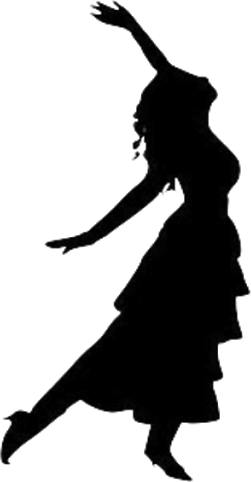
\includegraphics[height=45pt]{images/hiszpanska-dziewczyna.png}}
\begin{song}{title={Hiszpańskie dziewczyny}, music={tradycyjna angielska (Spanish Ladies)}, lyrics={Ryczące Dwudziestki}, capo={2}, annex}
    \begin{intro}
        Żegnajcie nam dziś, hiszpańskie dziewczyny \\
        Żegnajcie nam dziś, marzenia ze snów \\
        Ku brzegom angielskim już rzuszać nam pora \\
        Lecz kiedyś na pewno wró^{F#7}cimy tu z^{h}nów
    \end{intro}
    \begin{chorus}
        I s^{h}mak waszych ust, hiszpańskie dziew^{f#}czyny \\
        W noc ^{h}ciemną i złą nam będzie się ^{A}śnił \\
        Le^{G}niwie pop^{A}łyną znów ^{D}rejsu go^{h}dziny \\
        Wspom^{G}nienie ust waszych przys^{F#7}porzy nam ^{h}sił $\times 2$
    \end{chorus}
    \begin{verse}
        Nie^{h}długo ujrzymy znów w dali Cape ^*{f#}Dead man\footnotemark{} \\
        I Gł^{h}owę Baranią\footnotemark{} sterczącą wśród wz^{A}górz \\
        I s^{G}tatki sto^{A}jące na ^{D}redzie przed ^{h}Plymouth \\
        Kla^{G}rować kotwicę naj^{F#7}wyższy czas ^{h}już
    \end{verse}
    \begin{chorus}
        I smak waszych ust, hiszpańskie dziewczyny\ldots $\times 2$
    \end{chorus}
    \begin{verse}
        I znów białe żagle na masztach rozkwitną \\
        Kurs szyper wyznaczy do Portland i Wight\footnotemark{} \\
        I znów stara łajba potoczy się ciężko \\
        Przez fale, w kierunku na Beachy, Fairlight\footnotemark{}
    \end{verse}
    \begin{chorus}
        I smak waszych ust, hiszpańskie dziewczyny\ldots $\times 2$
    \end{chorus}
    \begin{verse}
        Zabłysną nam bielą skał zęby pod Dover \\
        I znów noc w kubryku wśród legend i bajd \\
        Powoli i znojnie tak płynie nam życie \\
        Na wodach i w portach South Foreland Light\footnotemark{}
    \end{verse}
    \begin{chorus}
        I smak waszych ust, hiszpańskie dziewczyny\ldots $\times 2$
    \end{chorus}
    \footnotetext{Dodman Point, Kornwalia; nie mylić z Cape Diamond, Quebec City --- to po innej stronie oceanu}
    \footnotetext{Ram Head, Kornwalia}
    \footnotetext{Isle of Wight (\textipa{/waIt/})}
    \footnotetext{Beachy Head i Fairlight, East Sussex}
    \footnotetext{wiktoriańska latarnia morska w South Foreland, Kent; nie ustalono, co autor miał na myśli}
\end{song}

